%reset references counter
\setcounter{NAT@ctr}{-1}
\cleartorightpage
\chapter*{}\label{chapter:tiaas}
\phantomsection\addcontentsline{toc}{section}{Planemo}

\begin{figure}[t!]
\centering

\includegraphics[height=10em]{chapters/platform/planemo.png}
\end{figure}
\vspace{-4cm}

\begin{changemargin}{0cm}{2cm}
\articletitle{Planemo: a command-line toolkit for developing, deploying, and executing scientific data analyses}
\end{changemargin}

Simon Bray\textsuperscript{\ref{planemo-affil:1}},
Matthias Bernt\textsuperscript{\ref{planemo-affil:2}},
Nicola Soranzo\textsuperscript{\ref{planemo-affil:3}},
Marius van den Beek\textsuperscript{\ref{planemo-affil:4}},
Bérénice Batut\textsuperscript{\ref{planemo-affil:1}},
Helena Rasche\textsuperscript{\ref{planemo-affil:5}},
Martin Čech\textsuperscript{\ref{planemo-affil:6}},
Peter Cock\textsuperscript{\ref{planemo-affil:7}},
Anton Nekrutenko\textsuperscript{\ref{planemo-affil:4}},
Björn Grüning\textsuperscript{\ref{planemo-affil:1}}
John Chilton\textsuperscript{\ref{planemo-affil:4}}

\textbf{Published in:} \emph{BioarXiv} March 2022,  \\

\doi{10.1101/2022.03.13.483965 }

\small

\begin{enumerate}
\itemsep-0.5em
\item Bioinformatics Group, Department of Computer Science, Albert-Ludwigs-University Freiburg, Georges-Köhler-Allee 106, 79110 Freiburg, Germany\label{planemo-affil:1}
\item Department of Computational Biology, Helmholtz Centre for Environmental Research GmbH - UFZ, Permoserstraße 15, 04318 Leipzig, Germany\label{planemo-affil:2}
\item Earlham Institute, Norwich Research Park, Norwich, NR4 7UZ, UK\label{planemo-affil:3}
\item Department of Biochemistry \& Molecular Biology, The Pennsylvania State University, University Park, PA, USA\label{planemo-affil:4}
\item Department of Pathology and Clinical Bioinformatics, Erasmus Medical Center, Wytemaweg 80, 3015 CN, Rotterdam, The Netherlands.\label{planemo-affil:5}
\item Institute of Organic Chemistry and Biochemistry, Prague, Czech Republic\label{planemo-affil:6}
\item James Hutton Institute, Invergowrie, Dundee DD2 5DA, UK\label{planemo-affil:7}
\end{enumerate}


§ These authors contributed equally to this work.
\dag Deceased

\section*{Abstract}
There are thousands of well-maintained high-quality open-source software
utilities for all aspects of scientific data analysis. For over a
decade, the Galaxy Project has been providing computational
infrastructure and a unified user interface for these tools to make them
accessible to a wide range of researchers. In order to streamline the
process of integrating tools and constructing workflows as much as
possible, we have developed Planemo, a software development kit for tool
and workflow developers and Galaxy power users. Here we outline
Planemo's implementation and describe its broad range of functionality
for designing, testing and executing Galaxy tools, workflows and
training material. In addition, we discuss the philosophy underlying
Galaxy tool and workflow development, and how Planemo encourages the use
of development best practices, such as test-driven development, by its
users, including those who are not professional software developers.
Planemo is a mature project widely used within the Galaxy community
which has been downloaded over 80,000 times.

The authors have declared no competing interest.

\url{https://github.com/galaxyproject/planemo}

\url{https://planemo.readthedocs.io}


\section*{Introduction}

The Galaxy project provides web browser access to command-line
scientific software, together with the necessary compute resources, in a
convenient, shareable and reproducible way, to researchers around the
world {[}1{]}. Over eight thousand tools are available for installation
onto any Galaxy server; users can run these individually, connect
multiple tools together to form workflows, and finally perform complex
analyses, without the need to access a command line. While Galaxy itself
does not require any significant computational skills to use,
development and maintenance of new tools and workflows benefit from
sophisticated infrastructure with both human and automated components.
The process of integrating software into Galaxy requires knowledge of
both the command-line interface of the underlying software and the
schema used by Galaxy to define tools, in order to be able to write a
`Galaxy tool wrapper' mapping dataset inputs, parameter inputs and
outputs between them. Once written, wrappers, as well as other Galaxy
artifacts such as workflows or training material {[}2{]}, are amenable
to routine processes such as testing, deployment and regular updates,
all of which can be automated using continuous integration (CI) systems.
Here we present Planemo, a versatile library and command line
application which is used extensively as a software development kit by
Galaxy or Common Workflow Language (CWL) {[}3{]} tool, workflow and
training material developers, and as a toolkit for Galaxy `power users'.
Planemo provides a simple but powerful command-line interface for tool
and workflow development and deployment, which encourages and enforces
good practices for software development. In addition, it enables
automated deployment of developed tools and automatic updates of the
software dependencies used internally by each Galaxy tool. The testing
functionality included in Planemo has been successfully integrated into
CI workflows of the major tool and workflow repositories, which helps to
ensure the creation of high quality tool wrappers and workflows.

Planemo is structured into numerous subcommands, which provide a broad
range of functionality. Here we discuss a selection of the most
important functionalities, grouped around the following themes: 1)
development of Galaxy tools, workflows, tutorials, and CWL tools; 2)
deployment of the developed tools and workflows; 3) automated tool and
workflow dependency updates and 4) tool and workflow execution.
\protect\hypertarget{xref-table-wrap-1-1}{\protect\hyperlink{tbl1}{Table
1}} summarizes this functionality, and
\protect\hypertarget{xref-fig-1-1}{\protect\hyperlink{fig1}{Fig. 1}}
provides a graphical overview. In addition to its use as a command-line
application, Planemo can also be used as a library by other projects. An
example is the Planemo Training Development Kit project
(\protect\hypertarget{ext-link-4}{\url{https://github.com/galaxyproject/ptdk}}),
which provides Planemo's functionality for creating training material
for Galaxy workflows via a webserver.

\hypertarget{tbl1}{}
biorxiv;2022.03.13.483965v1/TBL1

T1

tbl1

Overview of Planemo functionality and subcommands. Columns represent
artifacts that can be created or manipulated with Planemo, rows
represent different actions that can be performed on them. Italics
represent actions which are performed without using Planemo: trainings
are deployed using Jekyll and executed by users following the training
material in the graphical interface.

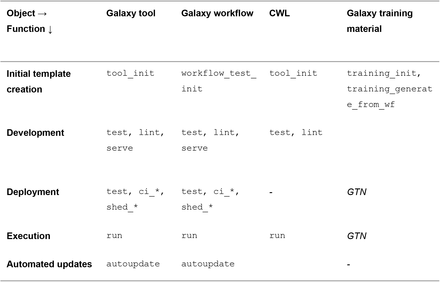
\includegraphics[width=0.5\textwidth]{chapters/images/planemo/T1.medium.png}

\begin{figure}
\hypertarget{fig1}{%
\centering
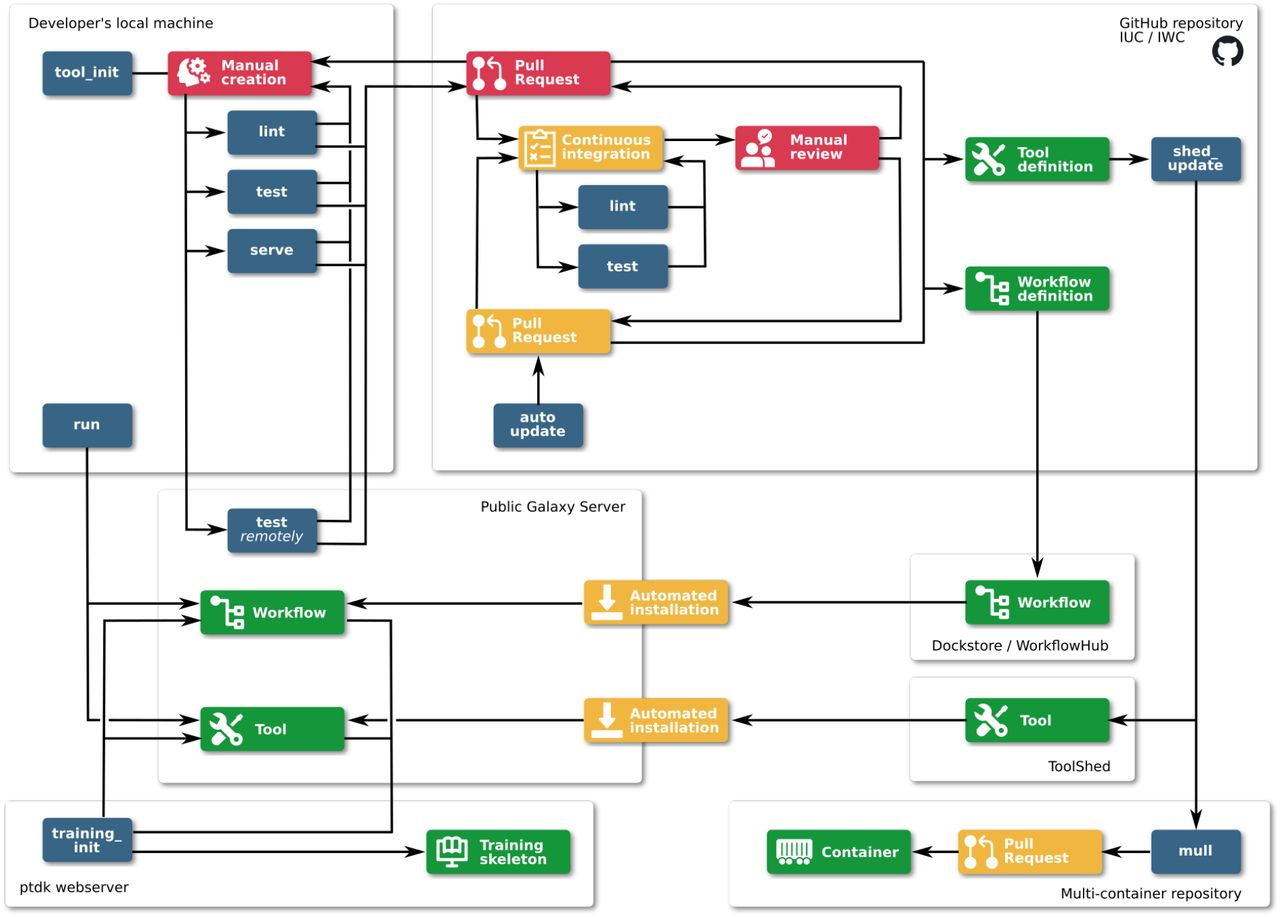
\includegraphics[width=\textwidth]{chapters/images/planemo/F1.large.jpg}
\caption{Overview of the use of Planemo for development, deployment, and
execution of Galaxy tools, workflows and training materials. Red =
manual work, blue = Planemo commands, yellow = automated steps, green =
created artifacts.}\label{fig1}
}
\end{figure}

\section*{Methods}

\subsection*{Software design}

Planemo is implemented as a Python package and distributed via GitHub,
PyPI and Bioconda {[}4{]}. As already described in the Introduction,
Planemo is a highly flexible, multifunctional software, which can be
used for: 1) different types of artifacts (e.g. tools, workflows), 2)
different workflow/tool languages and management systems (e.g. Galaxy,
CWL), 3) different tasks (e.g. linting, testing, executing). To handle
this variety, Planemo defines two central abstractions: Runnables and
Engines. Runnables include tools and workflows written for either Galaxy
or CWL; an Engine provides access to an external piece of software (such
as Toil or Galaxy) capable of executing a particular Runnable. Each
Engine has various methods (e.g. run(), test()), which define a
particular interaction with a Runnable.

Engines are provided for both local and external Galaxy servers, as well
as for cwltool {[}5{]} and Toil {[}6{]}. These interact with their
respective workflow management systems via the cwltool and Toil Python
modules (for CWL), and via the BioBlend library {[}7{]}, which provides
access to the Galaxy API through Python. Numerous lower-level functions
and classes are provided to connect the Engines with the underlying
functionality.

Some tasks cannot be easily described in the context of these
abstractions; for example, linting of tool or workflow definitions
requires only that the structured document containing the definition be
compared with a schema. Other examples include the functionality for
automatic updates of software dependencies and generation of training
material. Planemo handles these cases using separate classes and
functions.

Planemo is most frequently used as a command-line application, using a
command-line interface written using the Click package to provide a
straightforward way to access the components described above. Multiple
subcommands expose some of the most important tasks a user might want to
perform. For example, a user could run
\texttt{‘planemo\ test\ tool.xml’} to test a Galaxy tool wrapper.
Planemo will detect the type of Runnable (Galaxy tool) represented by
the filepath and start the appropriate Engine (temporary local Galaxy
instance), execute the Runnable on it, collect the results, and compare
them to predefined test data to determine a pass or fail status. All
subcommands can be configured by appending flags and options.

\subsection*{Implementation of continuous integration jobs}

While Planemo is designed primarily with developers and users in mind,
commands often need to be executed as part of automated continuous
integration (CI) jobs -- for example, testing of newly created Galaxy
tools after submission to a GitHub repository. Galaxy tools and
workflows are hosted over multiple repositories; to ensure a unified
approach to testing, a GitHub CI action is provided. The CI workflow
consists of the following components:

1. Identifying modified tools and repositories using
\texttt{‘planemo\ ci\_find\_repos’} and
\texttt{‘planemo\ ci\_find\_tools‘}.

2. Linting of Galaxy tools using \texttt{‘planemo\ lint’}.

3. Testing the tools -- as this is the most time-consuming step, the
tools found are chunked and multiple jobs run in parallel.

4. Linting of Python and R scripts packaged together with the tools.

5. If the PR is approved and merged: deployment to the Toolshed with
`planemo shed\_update'.

\subsection*{Definition of terms}

Planemo's features rely on and are interdependent with a variety of
other subprojects within and related to the Galaxy community. We
therefore first outline a few of these.

\subsubsection*{IUC}

The Intergalactic Utilities Commission {[}8{]} maintains a central
repository of Galaxy tool wrappers, currently hosted on GitHub. New
wrappers are added by means of a GitHub pull request, reviewed by IUC
members, and are tested by automated CI. After approval, the tool is
automatically deployed to the Galaxy ToolShed. Tools are subject to
further automatic updates, as new versions of software dependencies are
released. The IUC serves as a model for smaller communities developing
wrappers for more specialized tools (for example, Galaxy-P {[}9{]} for
proteomics) and has developed a set of guidelines for tool development.

\subsubsection*{Bioconda/BioContainers}

Each Galaxy tool has certain dependencies, which are typically installed
either using the Conda package manager {[}10{]} or within a container
(Docker {[}11{]} or Singularity {[}12{]}). Development and maintenance
of the necessary Conda packages or containers is performed by the
Bioconda and Biocontainers {[}14{]} communities, which collaborate
closely with the Galaxy project.

\subsubsection*{ToolShed}

A central `app store' for Galaxy tools Any user can upload to the
ToolShed {[}13{]}, but most high-quality tools are developed
collaboratively on an open platform like GitHub (for example by the IUC)
and deployed automatically.

\subsubsection*{IWC}

maintains a set of curated workflows {[}14{]}, consisting of multiple
component Galaxy tools, which are hosted on GitHub and deployed to
Dockstore {[}15{]} and the Workflow Hub {[}16{]}, analogously to the
development and deployment of Galaxy tools to the ToolShed by the IUC.

\subsubsection*{Galaxy Training Network}

A repository for tutorials, each describing a method for data analysis
in Galaxy {[}1{]}. Each tutorial is made up of multiple steps and
therefore corresponds to a Galaxy workflow, which forms the skeleton
around which the tutorial is built.

\subsubsection*{Continuous Integration (Workflow)}

A workflow run remotely on a build server which tests and deploys Galaxy
artifacts developed. It should not be confused with a Galaxy workflow.

\subsubsection*{Tool}

Artifact defined by a tool wrapper and stored in the ToolShed, allowing
users to access the functionality of the underlying software via Galaxy.

\subsubsection*{Galaxy Tool Wrapper}

Structured document defining a Galaxy tool; it maps dataset inputs and
outputs and other parameters between the underlying command-line tool
and the Galaxy API.

\subsubsection*{Galaxy Workflow}

a directed acyclic graph in which nodes can be dataset inputs or
outputs, parameter inputs, or tools. More informally, a combination of
multiple individual tools into a single pipeline, which once assembled
can be executed as if it were a single tool.

\subsubsection*{Collection}

a group of individual datasets linked together in a directory-like
structure. When a tool is run on a collection, individual jobs are
generated for each of the datasets which make up the collection. In
combination with workflows, collections allow Galaxy users to scale up
analyses to deal with large sets of data.


\subsection*{Documentation}

Planemo's documentation is hosted on a ReadTheDocs site:
\protect\hypertarget{ext-link-5}{\url{https://planemo.readthedocs.io}}.
In addition, several tutorials are available as part of the Galaxy
Training Network:

\begin{itemize}
\item
  Creating Galaxy tools from Conda through deployment:
  \protect\hypertarget{ext-link-6}{\url{https://training.galaxyproject.org/training-material/topics/dev/tutorials/tool-from-scratch/tutorial.html}}
\item
  Creating training material with Planemo:
  \protect\hypertarget{ext-link-7}{\url{https://training.galaxyproject.org/training-material/topics/contributing/tutorials/create-new-tutorial/tutorial.html}}
\item
  Automating Galaxy workflows using the command line:
  \protect\hypertarget{ext-link-8}{\url{https://training.galaxyproject.org/training-material/topics/galaxy-interface/tutorials/workflow-automation/tutorial.html}}
\item
  Test-driven development with Planemo:
  \protect\hypertarget{ext-link-9}{\url{https://planemo.readthedocs.io/en/latest/writing_advanced.html\#test-driven-development}}
\end{itemize}

\section*{Results and Discussion}

\subsection*{Galaxy tool development}

A Galaxy tool is defined by a wrapper for an underlying software (or
code), which maps its dataset inputs, parameter inputs and outputs to a
command-line script executed by Galaxy. When running a tool in the
Galaxy interface, a user selects their preferred choices for the exposed
dataset and parameter inputs. The Galaxy server then constructs the
command, schedules it as a job onto appropriate compute resources,
collects the results once the job has completed, and returns them to the
user.

Writing Galaxy tool wrappers requires a thorough knowledge of the
underlying software and also an understanding of the Galaxy tool schema
which defines how Galaxy wrappers are written. The tool schema is
defined in a simple manner, in order to make the process of wrapping
software as accessible as possible {[}17{]}. Planemo provides several
helpful features which assist tool developers in creating high-quality
wrappers that meet community-defined standards, such as those {[}18{]}
developed by the Intergalactic Utility Commission (IUC). These features
are implemented as subcommands, e.g. `\texttt{planemo\ test}'. Planemo
also helps to enforce software development best practices such as
writing tests for all tools and linting the wrapper definitions to avoid
bugs and ensure a coherent and readable style. Further support for tool
development standards is provided by the Galaxy Language Server
{[}19{]}, an implementation of the Language Server Protocol {[}20{]} and
a Visual Studio Code extension for Galaxy tools, which can be used
side-by-side with Planemo.

A common starting point for tool development is the
`\texttt{tool\_init}' subcommand. To use this, the developer provides a
variety of options, including an example command line, tool name,
inputs, outputs and software requirements, from which Planemo generates
a skeleton tool wrapper. Most of the `\texttt{tool\_init}` parameters
are optional, but the more that are provided, the more detailed the
initial skeleton will be.

The developer can then inspect and edit the generated file, adding more
parameters and increasing the complexity of the wrapper logic by
incorporating conditionals and repeat elements if necessary. As they
continue to edit, they can use the `\texttt{lint}` subcommand to
validate the wrapper under development. Planemo's linting forces
wrappers to match Galaxy's tool schema, ensuring stylistic consistency
and preventing some errors such as mismatched file formats. Crucially,
Planemo recommends that wrappers define at least one test case to ensure
the development of high-quality, portable, reliable and functional
tools, and this recommendation is strictly enforced by the IUC's and
other tool repositories. Once tests are defined, together with an
initial tool definition, the developer can start to run the tests using
the `\texttt{test}` subcommand. This launches a transient Galaxy server
on the developer's computer, installs the Galaxy tool under development,
together with all software dependencies, and executes the tests
specified within the tool wrapper. The results of the tests are then
returned to the developer, by default using a report defined using JSON
and HTML, although other format types are also supported (xUnit, jUnit,
Markdown and Allure).

Planemo encourages the use of test-driven development {[}21{]}, a
software development principle which states test cases should be written
before a new feature is developed. Test-driven development is an
industry-wide best practice. Defining extensive test cases at the start
of the process covering the required features provides a focus for
development, and results in more robust and better documented code
containing fewer bugs. The tool developer is forced to adopt the
perspective of the Galaxy user from the start to consider possible
use-cases of the software for which tests need to be written. Initial
test failures lead to iterative refinement of the wrapper, until a
fully-functional Galaxy tool, which passes all tests, is produced.

Once tests are passing, the developer should optimize the tool interface
which is presented to the user of the tool. To facilitate this, Planemo
provides the `\texttt{serve}` subcommand, which launches a Galaxy server
with the new tool installed, allowing the developer to inspect the
rendering of the wrapper in the graphical interface and to perform
manual testing. The developer should also improve the documentation of
the tool, by annotating each of the tool parameters, as well as writing
a help section to explain the tool's aim and usage, which appears
beneath the tool parameters in the graphical interface.

\subsection*{Common Workflow Language tool development}

In addition to Galaxy tools, Planemo also acts as a software development
kit for CWL tools. The same subcommands described can be used for this
purpose, including `\texttt{tool\_init}' and `\texttt{test}'. By
appending the `\texttt{-\/-cwl}' argument to the `\texttt{tool\_init}'
subcommand, Planemo generates a template for a CWL tool definition,
rather than a Galaxy wrapper. The test and lint commands then detect
that the input file is a CWL wrapper and process it accordingly. Tools
are tested by executing with the CWL engine cwltool and comparing the
result with test data or specified assertions, in the same way as for
Galaxy tools. The completed wrapper can be run using any CWL engine,
such as cwltool, Toil, Arvados {[}22{]} or Galaxy.

\subsection*{Galaxy workflow development}

Workflows are created in Galaxy by connecting together multiple tools
(i.e. an output of one tool becomes an input for the following one) in
order to automate complex analyses. Unlike tools, workflows can be
defined and edited in Galaxy's graphical workflow editor; often the
starting point is an interactive analysis (a Galaxy history) from which
a workflow can be extracted automatically. It is also possible to
manually author workflows in the gxformat2 workflow language {[}23{]},
and the user can switch between manually writing workflows and editing
in the graphical interface using the `\texttt{workflow\_edit}'
subcommand, which spins up a Galaxy instance with the workflow under
development pre-installed for editing. Planemo additionally facilitates
the creation of test cases by providing the option of generating them
automatically from a pre-existing workflow invocation.

Once a draft version of the workflow exists, it should be iteratively
improved in the same way as for tools, using the same lint, test and
serve subcommands already introduced. The `\texttt{workflow\_lint}`
subcommand checks workflows for errors and conformance with best
practices---a command-line interface mirroring functionality which is
also provided by the Galaxy graphical workflow editor. For example,
workflows which are missing test cases, labeled outputs, or essential
metadata fail linting. Running the `\texttt{test}` subcommand launches a
local Galaxy instance, installs the tools used in the workflow, uploads
the workflow and executes it on the provided input test data. In the
same way as for tool testing, the workflow outputs are downloaded and
compared to the test data, resulting in either a pass or fail status. In
some cases, it can be convenient to run testing on an existing public
server, such as
\protect\hypertarget{ext-link-10}{\url{https://usegalaxy.org}},
\protect\hypertarget{ext-link-11}{\url{https://usegalaxy.eu}}, or
\protect\hypertarget{ext-link-12}{\url{https://usegalaxy.org.au}}; this
is also supported by Planemo. Running the `\texttt{serve}` subcommand
provides a local Galaxy server with the workflow and the needed tools
pre-installed, which can be used for workflow development and
fine-tuning.

\subsection*{The philosophy of Galaxy tool and workflow
development}

After the previous discussion of the process of tool and workflow
development, the question arises how software complexity should be
divided between the tool and the workflow level. Should most of the
effort go into developing workflows, keeping tools as simple as possible
and flexibly rewrapping the underlying software depending on the demands
of a particular workflow, or should developers invest time creating
complex and multifunctional tools which can be reused without
modification in multiple workflows?

Galaxy leans heavily towards the second of these two options, as does
CWL, though the following discussion will focus on Galaxy. Galaxy
encourages the creation of modular tools which are usable in isolation,
so they can be used interchangeably in multiple different workflows.
Tools generally encapsulate most of the complexity of the underlying
software, allowing workflows to be simply constructed in a graphical
interface by connecting the component tools. Workflows can thus be
thought of as complex structures built from the same fundamental
building blocks, which can be constructed without knowledge of the
internal functionality of the individual tools. This has several
advantages with regard to the user experience: building workflows
becomes a far less daunting task, and tools can also be used
individually in the graphical interface, which makes Galaxy accessible
to new users and enables its use as a teaching environment for
scientific analysis.

Another advantage of this approach is the ``separation of concerns'', a
design principle in computer science. Different groups of scientists can
develop and apply specialized and complementary areas of knowledge: the
tool developer can concentrate on describing and developing the Galaxy
tool, without considering any downstream workflows that will be created
later. On the other hand, the workflow developer can construct complex,
high-level pipelines, without the detailed understanding of the
component tools and the command-line possessed by the tool developer.
This has the dual advantage that workflows can be treated on a more
abstract level and that the workflow creation process is made accessible
for a far greater number of users.

Separation of concerns between tools and workflows also benefits
security. Executing untrusted software on a compute cluster is highly
undesirable; thus workflows need to be assessed for security risks
before execution. For many workflow management systems, this assessment
must be repeated for each workflow. By contrast, as the Galaxy tool
review process involves checking tools for security issues before
merging, a system administrator can deploy tools developed by the IUC or
similar high-trust communities with confidence. The question of workflow
security is thus made redundant: if the component tools are trusted, a
workflow based on those tools can likewise be trusted.

These advantages must be balanced against the time investment required
from community members to build up a diverse set of tools, to allow the
construction of scientifically interesting workflows. Nonetheless, the
Galaxy community, facilitated by Planemo, has succeeded in developing
such a toolset and making it available to the scientific community.

\subsection*{Continuous integration for community
repositories}

Galaxy has a large and vibrant community of tool and workflow
developers, creating Galaxy tools in a wide range of scientific fields,
ranging from genomics to proteomics, computational chemistry and climate
science. As a result, a large number of high quality tools already exist
and are actively maintained over several GitHub repositories, centered
around the main IUC repository; the IWC (see Methods for definition)
performs the equivalent function of a repository for Galaxy workflows.
Building these communities has required many years of work by multiple
contributors; in order to streamline the process and ease the burden on
the tool developers, developing infrastructure to facilitate human
review and automate as much as possible is essential. Planemo forms the
core of this infrastructure.

Once a developer has completed the tool wrapper or workflow, they can
submit it to a community repository, usually hosted on GitHub, for
review. Alternatively, they may also deploy it themselves (for example,
to the ToolShed or WorkflowHub), but submission to a community
repository is encouraged to ensure the code is thoroughly reviewed and
to publicize the new tool or workflow. Community repositories are
configured to run the linting and testing checks already described after
submission, via a continuous integration (CI) workflow. Planemo provides
a couple of simple subcommands, `\texttt{ci\_find\_repos}` and
`\texttt{ci\_find\_tools}`, to identify tools which have been added or
modified. Both of these allow chunking of tools in order to parallelize
the testing process over multiple CI jobs. As part of the CI testing,
linting and testing of the tools is repeated, as well as linting of any
Python and R scripts added together with the new tool wrappers. These
steps ensure the submitted tools are of high quality, enforce consistent
standards on the code and reduce the maintenance burden for the entire
community.

If all tests pass and the proposed new tool or workflow is accepted by
the community, another CI job is initiated to deploy it to the ToolShed.
This makes use of Planemo's `\texttt{shed\_update}` command, which uses
the ToolShed credentials associated with the repository to upload the
newly created tool. Once it is available on the ToolShed, it can easily
be installed onto any Galaxy server.

The entire process, consisting of automated testing, human review and
automated deployment, ensures the creation of high-quality, trustworthy
tools which can be safely installed and used. It requires several more
specialized steps, which go beyond the simple Planemo subcommands that
the developer runs on their local machine. To package these CI workflows
into a single unit, a GitHub Action is provided {[}24{]} which can be
reused in other tool repositories. New tool repositories with the same
structure as the IUC repository can be conveniently created from a
template repository created by the Galaxy community {[}25{]}.

\subsection*{Automation of tool and workflow updates}

Another feature offered by Planemo is automatic updates of Galaxy tool
and workflow software dependencies, using the \texttt{‘autoupdate‘}
subcommand. In combination with separate autoupdate features already
developed by the Bioconda and conda-forge {[}26{]} communities, this
forms a sequence of semi-automated software update procedures, which are
triggered by an official release of new source code. After this new
release appears, this chain ensures that new Conda packages, new Docker
and Singularity containers, updated Galaxy tools and finally updated
Galaxy workflows are generated
(\protect\hypertarget{xref-fig-2-1}{\protect\hyperlink{fig2}{Fig. 2}}).
At each step, a CI job detects the artifact published in the previous
step and initiates the process of updating a dependent artifact,
generally by means of a GitHub pull request (PR).

\begin{figure}
\hypertarget{fig2}{%
\centering
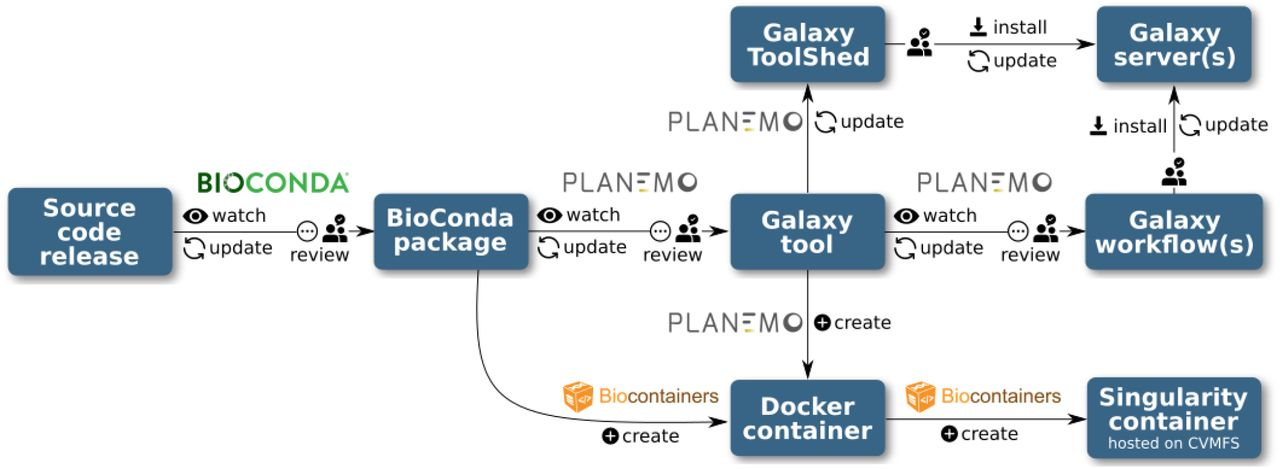
\includegraphics[width=\textwidth]{chapters/images/planemo/F2.large.jpg}
\caption{Automation pipeline for Bioconda packages, BioContainers,
Galaxy tools and workflows. Steps marked in red require human review;
steps marked in blue are fully automated.}\label{fig2}
}
\end{figure}

The CI pipelines developed by Bioconda and conda-forge monitor the Conda
recipes they maintain, regularly checking the links provided in the
recipes for new releases. When the developers of an upstream software
package release a new version, the CI creates a PR to update the package
recipe. Once the PR is reviewed and merged, newly built packages are
uploaded to the Anaconda repository.

In parallel, a bot {[}29{]} running the \texttt{‘autoupdate‘} subcommand
monitors the Galaxy tool wrappers maintained by the IUC, as well as a
few other smaller communities, checking the dependencies defined in the
tool wrapper. Once an updated Bioconda or conda-forge package is
published in the step above, the Planemo autoupdate bot detects this and
updates the dependencies section of the Galaxy tool accordingly. A PR is
then submitted to the GitHub repository, to be reviewed and manually
updated if necessary, before it is merged and deployed as described in
the ``CI for community repositories'' section.

Galaxy tools can specify multiple dependencies. If these dependencies
are installed via Conda, the packages can be simply installed into a
single environment, but if dependency installation is achieved using
containers, a new container must be built for each required combination
of dependencies. This is achieved by the `mulled build' infrastructure;
a CI job triggers the building of a Docker container for each new
combination of packages, on publication of new Galaxy tool versions.
Another CI job is responsible for generating Singularity containers from
the new Docker containers, which are made available by the BioContainers
and Galaxy communities via a CernVM file system (CVMFS) {[}27{]}. These
steps do not require manual review.

The Planemo autoupdate bot also monitors the Galaxy workflows maintained
by the IWC and checks whether new versions exist for each of the
component tools. Once a new tool version is created (either by the
upstream tool autoupdate step, or a tool developer), the workflow
definition file hosted by the IWC is modified accordingly and a PR
submitted for review
(\protect\hypertarget{xref-fig-3-1}{\protect\hyperlink{fig3}{Fig. 3}}).

\begin{figure}
\hypertarget{fig3}{%
\centering
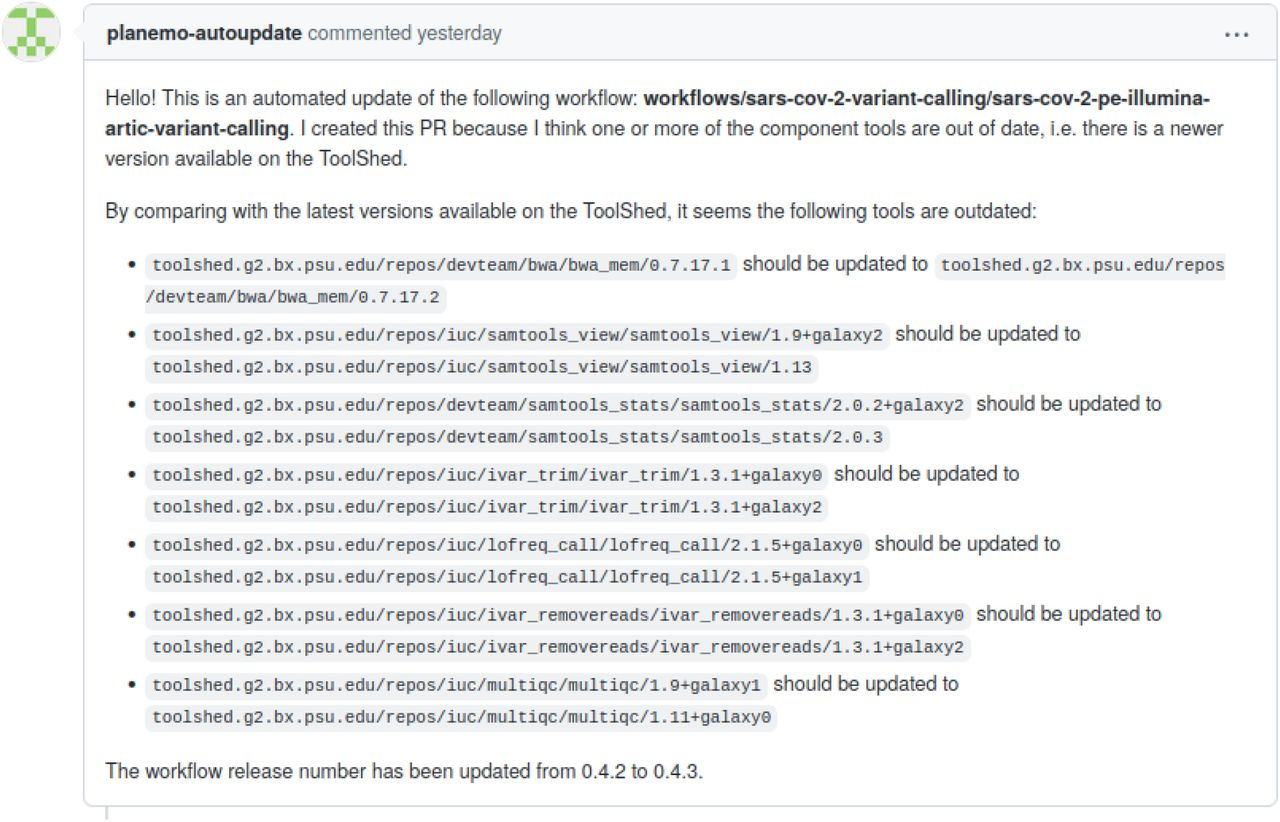
\includegraphics[width=\textwidth]{chapters/images/planemo/F3.large.jpg}
\caption{An example GitHub pull request created by the Planemo
autoupdate bot, updating a workflow hosted on the IWC.}\label{fig3}
}
\end{figure}

\subsection*{Execution}

Apart from providing assistance with tool and workflow development and
deployment, Planemo is also a useful resource for Galaxy power users who
need to launch high-throughput data analyses. Galaxy is traditionally
accessed via a graphical interface in the web browser, and features such
as Galaxy collections already provide a high level of parallelization to
users of the graphical interface. Nonetheless, there are important
scenarios in which a user might need to run individual workflows
hundreds or thousands of times, in which the data cannot be grouped into
collections ahead of time---for example, for variant calling of
SARS-CoV-2 genomic data, in which a huge amount of new data is published
continuously {[}28{]}. As a convenient alternative to the graphical
interface, Planemo allows workflow execution to be scheduled
programmatically using the `\texttt{run}` subcommand, either on a local
machine or a larger Galaxy server. `\texttt{planemo\ run}` can be
embedded in scripts of varying complexity, which can be scheduled and
controlled via CI systems or message queues to run workflows on demand -
such as on new data appearing or tool updates.

Internally, Planemo executes workflows by submitting them to the chosen
server via Galaxy's API. Requests to the API are made using BioBlend, a
library which wraps many API endpoints as Python methods. It is also
possible to execute workflows directly using BioBlend, or simply by
making API calls using a tool such as cURL. While this approach does
offer a high level of flexibility, it requires the user to possess a
high level of knowledge of the API (for example, the correct format to
submit workflow parameters) and often requires the creation of custom
scripts. By contrast, Planemo's `run` subcommand offers a high-level
interface to execute workflows, monitor them during execution, and
report on their status after completion, packaged as a single command.

For tool and workflow development, the artifacts under development are
generally tested against an ephemeral local Galaxy instance, which is
deleted after use. While this is also supported by the `\texttt{run}`
subcommand, with the workflow outputs saved to a specified location,
this approach is not scalable for workflows which demand long compute
times, with large data inputs, or with workflows which need to be
executed multiple times. In many cases, the user may prefer to make use
of established, stable infrastructures, such as a public Galaxy instance
or a private instance administered by their research group. Planemo
allows external Galaxy instances to be specified for all `\texttt{run}`
and `\texttt{test}` commands by providing the server URL and user API
authentication key on the command line. As it is inconvenient and
insecure to enter the API key with each command, Planemo also allows
users to define profiles, in which the URL and API key is configured for
each server. The user can then define multiple profiles and run
workflows on different servers simply by appending, e.g.
`\texttt{-\/-profile\ usegalaxy-org}` or
`\texttt{-\/-profile\ private-server}` to the command.

Planemo provides numerous command line options to configure the workflow
execution process. The name of the history in which the new invocation
is created, as well as a list of Galaxy tags to add, can be specified
via the command line. In addition, Planemo and Galaxy allow both
datasets and workflows to be specified via hexadecimal IDs which point
towards a Galaxy object on an external server, rather than by referring
to a local path. This has the advantage of avoiding multiple uploads of
the same dataset or workflow, if the workflow has to be executed
multiple times. Planemo can also be configured to either wait until the
workflow has completed, and download the output datasets created, or to
terminate once the workflow has been successfully scheduled. In the
latter case, the `\texttt{list\_invocations}` command can be used to
monitor running workflows and to return the number of jobs which have
succeeded, failed, or incomplete. If jobs have failed---for example, due
to transient server issues--- the user can also choose to restart them
using the `rerun` subcommand.

\subsection*{Training material}

Planemo provides utilities for developing tutorials for different types
of data analysis with Galaxy. The Galaxy Training Network, accessible
via
\protect\hypertarget{ext-link-13}{\url{https://training.galaxyproject.org}},
provides a range of training material including slide decks, tutorials
and videos. In particular, the tutorials are written in Markdown and
rendered using Jekyll, and often feature `hands-on boxes' which describe
the exact combination of parameters and input which users need to submit
when running a Galaxy tool. Most tutorials instruct the trainees to run
several Galaxy tools in sequence, and thus correspond to a Galaxy
workflow.

Planemo provides two subcommands, \texttt{‘training\_init‘} and
\texttt{‘training\_generate\_from\_wf‘}, which generate a directory
structure for a new tutorial, containing skeleton Markdown files
defining the tutorials. These files already contain sections and
hands-on boxes for each tool, with the tool inputs and parameters
predefined, ensuring a high level of consistency in the appearance and
quality of the tutorials produced. The training developer can then take
these templates and expand them with additional information, questions,
diagrams and citations to produce the completed training. They also need
to provide input datasets, which are usually stored on Zenodo. To
populate a Galaxy server with these datasets, the training developer
should also provide a data library file, which can be generated using
the \texttt{‘training\_fill\_data\_library‘} subcommand, including the
Zenodo links and file formats of the datasets.

A major aim of the Galaxy Training Network project is improving
accessibility for new contributors, including for scientists who are not
comfortable with command-line software. As a result, the Planemo
functionality relating to training material development is provided in
webserver form as the Planemo Training Development Kit (PTDK). The
application is written using Flask and deployed with Heroku; it can be
accessed via
\protect\hypertarget{ext-link-14}{\url{https://ptdk.herokuapp.com}}. The
interface allows the selection of the same options as the Planemo
commands, with the additional option of specifying a workflow for
generating the training using its ID from one of the major public Galaxy
servers.

\section*{Conclusion}

We have presented Planemo, a library and application which has already
achieved widespread usage among Galaxy tool, workflow and training
material developers, Galaxy power users, and as part of numerous
automated deployment solutions. Planemo provides the developers of
command-line software with an easy way to create a graphical interface,
taking advantage of the many features developed by the Galaxy community
and the compute resources provided by public Galaxy instances. We have
described the complex infrastructure the Galaxy community has developed
for creating and interacting with artifacts such as tools, workflows and
training material. Planemo plays the crucial role of bridging the gaps
between the human and automated components of this infrastructure,
freeing members of the community to devote their time to developing,
reviewing and performing novel scientific analyses.

The authors are grateful to the broader Galaxy community for their
support and software development efforts. This work is funded by NIH
Grants U41 HG006620 and NSF ABI Grant 1661497. Usegalaxy.eu is supported
by the German Federal Ministry of Education and Research grants
031L0101C and de.NBI-epi to BG. Usegalaxy.org.au is supported by
Bioplatforms Australia and the Australian Research Data Commons through
funding from the Australian Government National Collaborative Research
Infrastructure Strategy. The funders had no role in study design, data
collection and analysis, decision to publish, or preparation of the
manuscript.


\footnotesize
\bibliographystyle{ieeetr}
\bibliography{references}
\normalsize
